\chapter{从发电厂到家中：交流发电机}\label{ch:g9:alternator}

一整年的千瓦时已经流经你的
能量审计表——可它们从何而来？顺着电缆走出房子，
穿过街道，跨越高压塔架，它的终点是一台
在大厅里旋转的机器：交流发电机。它的秘密是
本书电学中最动人的一个惊喜：
去年“电流生磁”的发现，反过来用。

\section{电磁感应：效应反过来}

\begin{proposition}[电磁感应]\label{prop:g9:alternator:induction}
把磁铁移近闭合电路——或把电路移近磁铁——
只要运动持续，就会出现电压，
并驱动电流：电是由磁场变化\emph{感应}出来的，
规则如下，均来自实验台：
\begin{enumerate}
  \item 只有\emph{变化}才能感应：静止的磁铁在
        线圈旁，什么也不产生——不论磁铁多强；
  \item 运动越快、磁铁越强、线圈匝数越多，
        感应电压越大；
  \item 运动反向，感应电流也反向——
        靠近与远离，电流的方向相反。
\end{enumerate}
去年是电流产生磁场；今年
则是运动的磁场产生电流。这两种效应
是同一枚硬币的两面——第二面
为文明提供动力。
\end{proposition}

\begin{method}[实验台上的感应]\label{met:g9:alternator:bench}
一个多匝线圈、一块条形磁铁、
一只零点居中的灵敏电流计：
\begin{enumerate}
  \item 将电流计接在线圈两端，把磁铁
        静置于线圈内：指针停在零点——
        仅仅磁性的强弱不会产生感应；
  \item 把磁铁推入线圈：指针向一侧偏转——
        运动一停，指针立即回到零点；
  \item 把磁铁抽出：指针同样偏转，但方向相反；
  \item 推得更快，偏转更大。把磁铁前后
        有节奏地来回抖动，指针先左、
        再右、再左——你正用手摇出交变
        电流。
\end{enumerate}
\end{method}

\begin{omfigure}
\begin{tikzpicture}[scale=0.85]
  \draw[thick, fill=omThm, fill opacity=0.5]
    (0.4,1.2) rectangle (2.6,2.0);
  \node[font=\small] at (1.5,1.6) {N \quad S};
  \draw[-Stealth, very thick, omExo] (2.9,1.6) -- (4.0,1.6);
  \foreach \x in {4.4,4.8,...,6.8} {
    \draw[very thick, omDef] (\x,0.9) arc (200:340:0.32 and 0.75);
  }
  \draw[thick, omDef] (4.4,0.9) -- (4.1,0.2);
  \draw[thick, omDef] (7.4,0.9) -- (7.7,0.2);
  \draw[thick] (4.1,0.2) -- (4.1,-0.4) -- (5.2,-0.4);
  \draw[thick] (7.7,0.2) -- (7.7,-0.4) -- (6.1,-0.4);
  \draw[thick, fill=white] (5.65,-0.4) circle (0.45);
  \draw[-Stealth, very thick, omThm] (5.65,-0.4) -- ++(60:0.38);
  \node[right, font=\small] at (7.9,1.6)
    {推入磁铁：指针偏转};
  \node[right, font=\small] at (7.9,1.0)
    {磁铁静置：指针不动};
\end{tikzpicture}

{\small 实验台上的感应：只有\emph{运动的}磁铁
才能唤醒线圈——指针偏转的方向随
运动方向而反转。}
\end{omfigure}

\section{交流发电机}

\begin{definition}[交流发电机]\label{def:g9:alternator:alternator}
\emph{交流发电机}\index{交流发电机}，是让感应
永不停歇的装置：磁铁稳定地在固定线圈旁转动（或线圈在磁场中转动）。
每转半圈，一个磁极靠近线圈，
随后又被带走——变化无穷无尽，不断更新——
于是感应电压依次为正、负、正，
按构造即是\emph{交变}的，
正好描绘出示波器那一章中平滑的正弦曲线。若
每秒转 50 圈，输出便以
\qty{50}{Hz} 交替变化：电网的频率\emph{正是}一个转速，
由电网上的每座电站共同保持同步。
\end{definition}

\begin{example}[车轮上的发电机]\label{ex:g9:alternator:dynamo}
自行车发电机是一台小型交流发电机：车轮带动
固定线圈内的一小块磁铁转动，车灯便亮起——
你蹬得越用力，灯越亮，频率也越高，
正如实验台规则所预言的（慢速骑行时灯光忽明忽暗，
正如交变电流一章所观察的）。它的代价也很真实：
发电机会拖慢车轮——点亮车灯要耗费你腿上的真实力气。
感应本身不提供能量；它只是把运动\emph{转化}为电能，
一焦耳换一焦耳，只是要扣掉摩擦力收取的“税”。
\end{example}

\begin{omfigure}
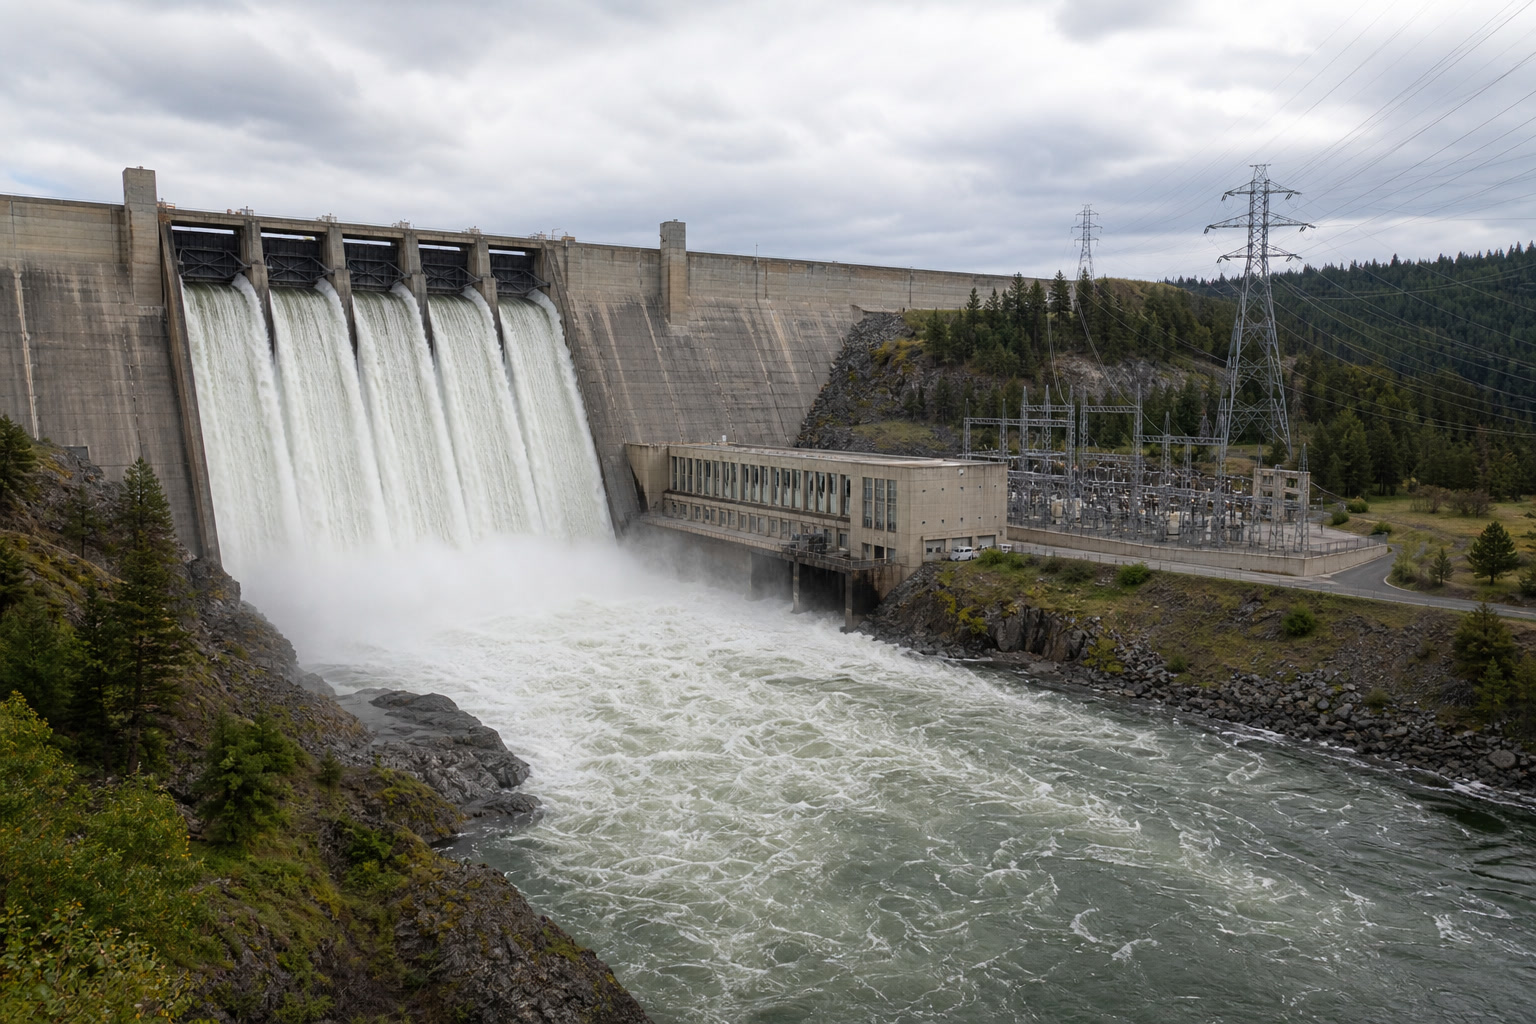
\includegraphics[width=0.55\linewidth]{images/book1/ai/g9-alternator-dam.jpg}

{\small 水电站：高处的水奔流而下，推动水轮机，交流发电机再把能量沿输电线送出。}
\end{omfigure}

\section{每座发电厂都是同一台机器}

\begin{proposition}[共同核心]\label{prop:g9:alternator:core}
世界上几乎所有的电，不论宣传上怎样说，
都是以同一方式产生的：某物使一个
\emph{涡轮}——一种坚固的叶片式风车——被推动，
而涡轮又带动交流发电机。发电厂的差别只在于
\emph{是什么在推动叶片}：
\begin{enumerate}
  \item 火力发电厂用燃烧煤炭或天然气
        烧开水——蒸汽喷流推动涡轮；
  \item 核电厂则用原子裂变
        所释放的热量烧水——仍是蒸汽；
  \item 水力发电大坝让山湖之水落下，
        冲过叶片——童年时那条水坝链，此刻补全了。
  \item 风力涡轮机省去了中间环节：风本身就是
        叶片的推动力，每个机舱里都有一台交流发电机。
\end{enumerate}
一个例外印证了这一规律：太阳能电池板发电，
完全无需转动——依靠的是一种光效应，
这属于大学阶段的内容。
\end{proposition}

\begin{omfigure}
\begin{tikzpicture}[scale=0.8]
  \node[draw, thick, omExo, font=\footnotesize, align=center,
    minimum width=2.1cm, minimum height=0.95cm] (src) at (0.9,0)
    {火焰、原子、\\湖水或风};
  \node[draw, thick, omMeth, font=\footnotesize, align=center,
    minimum width=1.9cm, minimum height=0.95cm] (tur) at (3.8,0)
    {涡轮机\\（转动！）};
  \node[draw, thick, omThm, font=\footnotesize, align=center,
    minimum width=2.0cm, minimum height=0.95cm] (alt) at (6.6,0)
    {交流发电机\\（电磁感应）};
  \node[draw, thick, omDef, font=\footnotesize, align=center,
    minimum width=2.0cm, minimum height=0.95cm] (gri) at (9.5,0)
    {变压器\\与电网};
  \draw[-Stealth, very thick] (src) -- (tur);
  \draw[-Stealth, very thick] (tur) -- (alt);
  \draw[-Stealth, very thick] (alt) -- (gri);
  \node[below, font=\footnotesize] at (2.35,-0.75) {热量或运动};
  \node[below, font=\footnotesize] at (5.2,-0.75) {转动};
  \node[below, font=\footnotesize] at (8.05,-0.75)
    {交流电};
\end{tikzpicture}

{\small 每座电站只有一条链：某物使涡轮机转动，
涡轮机带动交流发电机转动，电磁感应
完成其余部分。只有第一个方框因电站而异。}
\end{omfigure}

\begin{example}[核对后的能量链]\label{ex:g9:alternator:chains}
用专业术语，把每座电站写成一条童年时的能量链。
水坝：储存的高度 $\to$ 落水的运动
$\to$ 转动 $\to$ 电能 —— 太阳，别忘了，
曾通过蒸发把那湖水抬起：水力发电
不过是被推迟了的阳光。燃煤电厂：化学能储存
$\to$ 热量 $\to$ 蒸汽的运动 $\to$ 转动 $\to$
电能 —— 每个箭头处都有热量外泄，
正如冷却塔的烟羽所供认的。风力：流动的空气（由太阳搅动）
直接带动转动。大自然会不断补充的能源——水、风、阳光——
被称为
\emph{可再生的}\index{可再生的}；
被烧掉和裂变的储存，在人类的时间尺度上将永远耗尽。
\end{example}

\begin{remark}[为什么输电塔在 400000 伏时嗡嗡作响]\label{rem:g9:alternator:transport}
交流一章许下的最后一个承诺现在兑现。一座
城镇需要比如一亿瓦特的功率。由 $P = U I$，此功率
既可以用极大的电流、适中的电压输送，
也可以用较小的电流、极高的电压输送。但导线会随\emph{电流}发热
（即旧的热效应），输电塔每升温一度，都是
花了钱却被“乌鸦”白白拿走的能量。因此
电网以惊人的高电压输电——
即数十万伏、小电流、损耗极低，
再一个街区一个街区地降压——
降到你家墙上那温和的 \qty{230}{V}。负责降压的
机器，即\emph{变压器}，由两个线圈和
电磁感应再次登场——它只对交变的
电流起作用：整个电网采用交流电，
是因为变压器只能处理交流电。
\end{remark}

\section{练习}

\begin{exercise}[$\star$]\label{exo:g9:alternator:1}
陈述电磁感应的三条实用规则。一块
强磁铁\emph{静止}时会感应出什么？
\end{exercise}

\begin{exercise}[$\star$]\label{exo:g9:alternator:2}
交流发电机的输出为何会交变？请把正负号的
变化与转动联系起来。
\end{exercise}

\begin{exercise}[$\star$]\label{exo:g9:alternator:3}
交流发电机以多大的转速向一个
\qty{50}{Hz} 的电网供电？网络中的每个电站
因此必须就什么达成一致？
\end{exercise}

\begin{exercise}[$\star$]\label{exo:g9:alternator:4}
说出每座电厂都有的两个通用方框，以及
在燃煤、核能、水电与风电之间变化的那个方框。
\end{exercise}

\begin{exercise}[$\star$]\label{exo:g9:alternator:5}
写出从山湖到你
台灯的水力发电能量链——并说出注满
这湖水的那台天体“机器”。
\end{exercise}

\begin{exercise}[$\star$]\label{exo:g9:alternator:6}
为什么发电机的灯一亮，踩踏板
就会变费力？哪一条原理说明它不可能是别的样子？
\end{exercise}

\begin{exercise}[$\star$]\label{exo:g9:alternator:7}
将下列对象分为“可再生的”与“不可再生的”两类：风；煤；水坝的湖水；
铀；阳光。什么标准决定了这样的分类？
\end{exercise}

\begin{exercise}[$\star$]\label{exo:g9:alternator:8}
为什么电网要以数十万
伏的高电压输送电能？说出提供这一选择的公式，以及
决定这一选择的效应。
\end{exercise}

\begin{exercise}[$\star\star$]\label{exo:g9:alternator:9}
一台用手摇动的演示用交流发电机，若转得很慢，
灯会微弱且明显闪烁；若转得很快，灯会明亮
而稳定。请运用实用规则和
频率一章的内容解释这两种变化。
\end{exercise}

\begin{exercise}[$\star\star$]\label{exo:g9:alternator:10}
一座电站输出 \qty{1e8}{W}。比较
在 \qty{230}{V} 与 \qty{400000}{V} 下所需的电流（用
科学计数法）。实际电缆能承载哪一种？
\end{exercise}

\begin{exercise}[$\star\star$]\label{exo:g9:alternator:11}
火电站与核电站，本质上都是精巧的
烧水壶。试用它们的能量链为这一说法辩护 --- 并
指出两者不同的那一个环节。
\end{exercise}

\begin{exercise}[$\star\star\star$]\label{exo:g9:alternator:12}
倒着走一遍这趟大旅程：今晚你房间的灯在
\qty{230}{V}下发光。逆着追溯其能量，经过每一个环节
--- 变压器、输电塔、交流发电机、涡轮机，以及你选定的一种
一次能源 --- 说出每一阶段的能量
形式，以及沿途的损耗。然后
用一句九年级水平的话回答童年时的那个问题：
你房间里的光最终来自何处？
\end{exercise}

\section{问题：电站的夜班}

\begin{problem}[{周末问题 --- 水电站的夜班；
感应、同步与风暴；
工程师的日志}]\label{pb:g9:alternator:1}
你跟随山谷大坝的夜班工程师 --- 上方是湖，
下方是小镇，交流发电机在两者之间嗡嗡作响。

\medskip\noindent\textbf{第一部分 --- 机房。}
\begin{enumerate}
  \item 工程师打开闸门，水流轰鸣着冲过
        三号水轮机，它的交流发电机仪表随之亮起。
        写出从湖泊到母线的能量链。
  \item 在交流发电机内部，哪些运动，哪些静止 ---
        为什么必须有东西运动？
  \item 电网以 \qty{50}{Hz} 运行。工程师
        盯着表盘，使三号水轮机恰好保持
        对应的转速。转速出错时，会出什么问题？
        （其电压的频率会怎样
        变化？）
  \item 一名实习生问，若转子中换用更强的磁铁，
        能否“白白”得到额外的功率？请纠正这一想法，
        说明发电机的真实代价。
\end{enumerate}

\medskip\noindent\textbf{第二部分 --- 小镇的需求。}
\begin{enumerate}[resume]
  \item 凌晨 03:00，小镇用电功率为 \qty{2e7}{W}。在
        输电线的 \qty{200000}{V} 电压下，
        电站输出的电流为多少？
  \item 同样的功率若在 \qty{230}{V} 下传输，
        需要多大电流 --- 比较结果说明了
        变压器的什么作用？
  \item 早上 07:00，烧水壶与取暖器开始工作：
        需求翻倍。工程师必须给涡轮机
        增加什么？若她供给得太少，
        电网的频率会怎样？（机器
        负载下会变慢，就像骑车人爬坡
        一样。）
  \item 电站的姐妹电站 --- 山脊上的风电场 ---
        风一停便退出运行。哪一个环节
        出了故障，哪些环节仍然完全
        正常？
\end{enumerate}

\medskip\noindent\textbf{第三部分 --- 风暴。}
\begin{enumerate}[resume]
  \item 闪电切断了一条输电线；断路器跳闸。
        工程师把电力转到邻近的
        线路上。电网的什么性质 ---
        即一张庞大的并联网络 --- 使得改线成为可能？
  \item 忙乱之中，仓库的灯光
        变暗发黄一分钟。请解释：什么下降了，
        仓库的电动机与灯泡曾短暂地
        供电不足？
  \item 黎明时分：日志必须向实习生解释，
        这一整夜的电能，追根溯源，
        本是阳光。起草这段两行的解释（湖泊、
        蒸发、降雨）。
  \item 按惯例，日志的最后一行：
        用一句话概括这一夜的物理 --- 运动、磁性，
        并把小镇清晨的烧水壶也包括在内。
\end{enumerate}
\end{problem}
